\documentclass[12pt]{article}
% ------------------------------------------------------------------------------
% Packages
% ------------------------------------------------------------------------------
\usepackage[utf8]{inputenc} % input encoding
\usepackage{framed} % for \framebox
\usepackage[english]{babel} % language support 
\usepackage[colorlinks=true, linkcolor=blue, urlcolor=blue, citecolor=blue, anchorcolor=blue]{hyperref} % hyperref package
\usepackage{amsthm, amsmath, amsfonts, mathtools, amssymb, bm} % Math packages
\usepackage{xcolor} % Color package
\usepackage[shortlabels]{enumitem} % Enumeration package
\usepackage{booktabs}
\usepackage{float}
\usepackage{cancel}

% ------------------------------------------------------------------------------
% Document Style
% ------------------------------------------------------------------------------

% Header ----------------------------------------------------------------------
\addtolength{\hoffset}{-2.25cm}
\addtolength{\textwidth}{4.5cm}
\addtolength{\voffset}{-2.5cm}
\addtolength{\textheight}{5cm}
\setlength{\parskip}{0pt}
\setlength{\parindent}{15pt}

\pagestyle{myheadings}

\setlength{\parindent}{0in}

\pagestyle{empty}
\makeatletter
\def\fps@figure{H}
\def\fps@table{H}
% ------------------------------------------------------------------------------

% ------------------------------------------------------------------------------
% New commands
% ------------------------------------------------------------------------------
\newcommand{\qiq}{\qquad \implies \qquad}
\newcommand{\qiffq}{\qquad \iff \qquad}
\newcommand{\qaq}{\qquad \textbf{and} \qquad}
\newcommand{\qoq}{\qquad \textbf{or} \qquad}

% ------------------------------------------------------------------------------
% New environments
% ------------------------------------------------------------------------------
\newtheorem*{theorem}{\color{red!60!black}Theorem}
\newtheorem{corollary}{\color{blue}Corollary}
\counterwithin*{corollary}{subsection}
\newtheorem{lemma}{\color{blue}Lemma}
\counterwithin*{lemma}{subsection}
\newtheorem{proposition}{\color{blue}Proposition}
\counterwithin*{proposition}{subsection} 
\theoremstyle{definition}
\newtheorem*{definition}{\color{green!60!black}Definition}
\newtheorem{example}{\color{orange!80!black}Example}
\newtheorem*{Obs}{\color{purple!80!white}Observation}
\newtheorem*{As}{\color{red!80!white}Assumptions}
\newtheorem*{answer}{\color{red!60!white}Answer}
\newtheorem*{Cor}{\color{blue!60!white}Corollary}
\newtheorem{exercise}{\color{blue!60!white}Exercise}
\newtheorem{subexercise}{ \color{blue!40!white}  }[exercise]

\begin{document}
\title{Problem Set 1 }
\author{Mitchell Valdes-Bobes}
\maketitle
% \begin{abstract}
% 	We examine [X]
% \end{abstract}
% \thispagestyle{empty}

% \pagebreak{}
% This paper .... 


\section{Data}

For this section I started by selecting a sub-sample of the data that meet the following criteria:
\begin{itemize}
    \item Observation is from the \textbf{Main Sample} not from the \textbf{SEO oversample}.
    \item Year is between \textbf{1978} and \textbf{1997}.
    \item Age is between $\textbf{25}$ and $\textbf{25+35}$.
\end{itemize}

To remove possible outliers I removed all individuals that earned less than $\textbf{\$2000}$ or more than $\textbf{\$170000}$ for three straight years. 

\begin{center}
\begin{table}[h!]\caption{Summary Statistics for Selected Years}
\begin{tabular}{lrrrrr}
\toprule
{} &          1980 &          1983 &          1986 &          1989 &          1992 \\
\midrule
Household id      &   3206.483643 &   3249.745605 &   3250.229004 &   3516.174805 &   3886.425537 \\
Age               &     30.953697 &     31.883293 &     32.431976 &     32.982773 &     33.958717 \\
Spouse in HH      &      0.176914 &      0.198222 &      0.198342 &      0.198084 &      0.211662 \\
Household Size    &      3.516354 &      3.432950 &      3.415822 &      3.394453 &      3.344012 \\
Annual Work Hours &    923.329886 &    888.681067 &    959.502405 &   1003.831467 &    988.638406 \\
After-tax Income  &  18672.299583 &  22468.653739 &  27110.260518 &  34123.840211 &  38196.020521 \\
HS dropout        &      0.268782 &      0.252113 &      0.219807 &      0.201507 &      0.186769 \\
HS graduate       &      0.402462 &      0.400612 &      0.380790 &      0.380268 &      0.380933 \\
White             &      0.878611 &      0.879812 &      0.881998 &      0.883712 &      0.885025 \\
\bottomrule
\end{tabular}

\end{table}
\end{center}

After this transformation the distribution of income looked like 
\begin{figure}[h*]
    \centering
    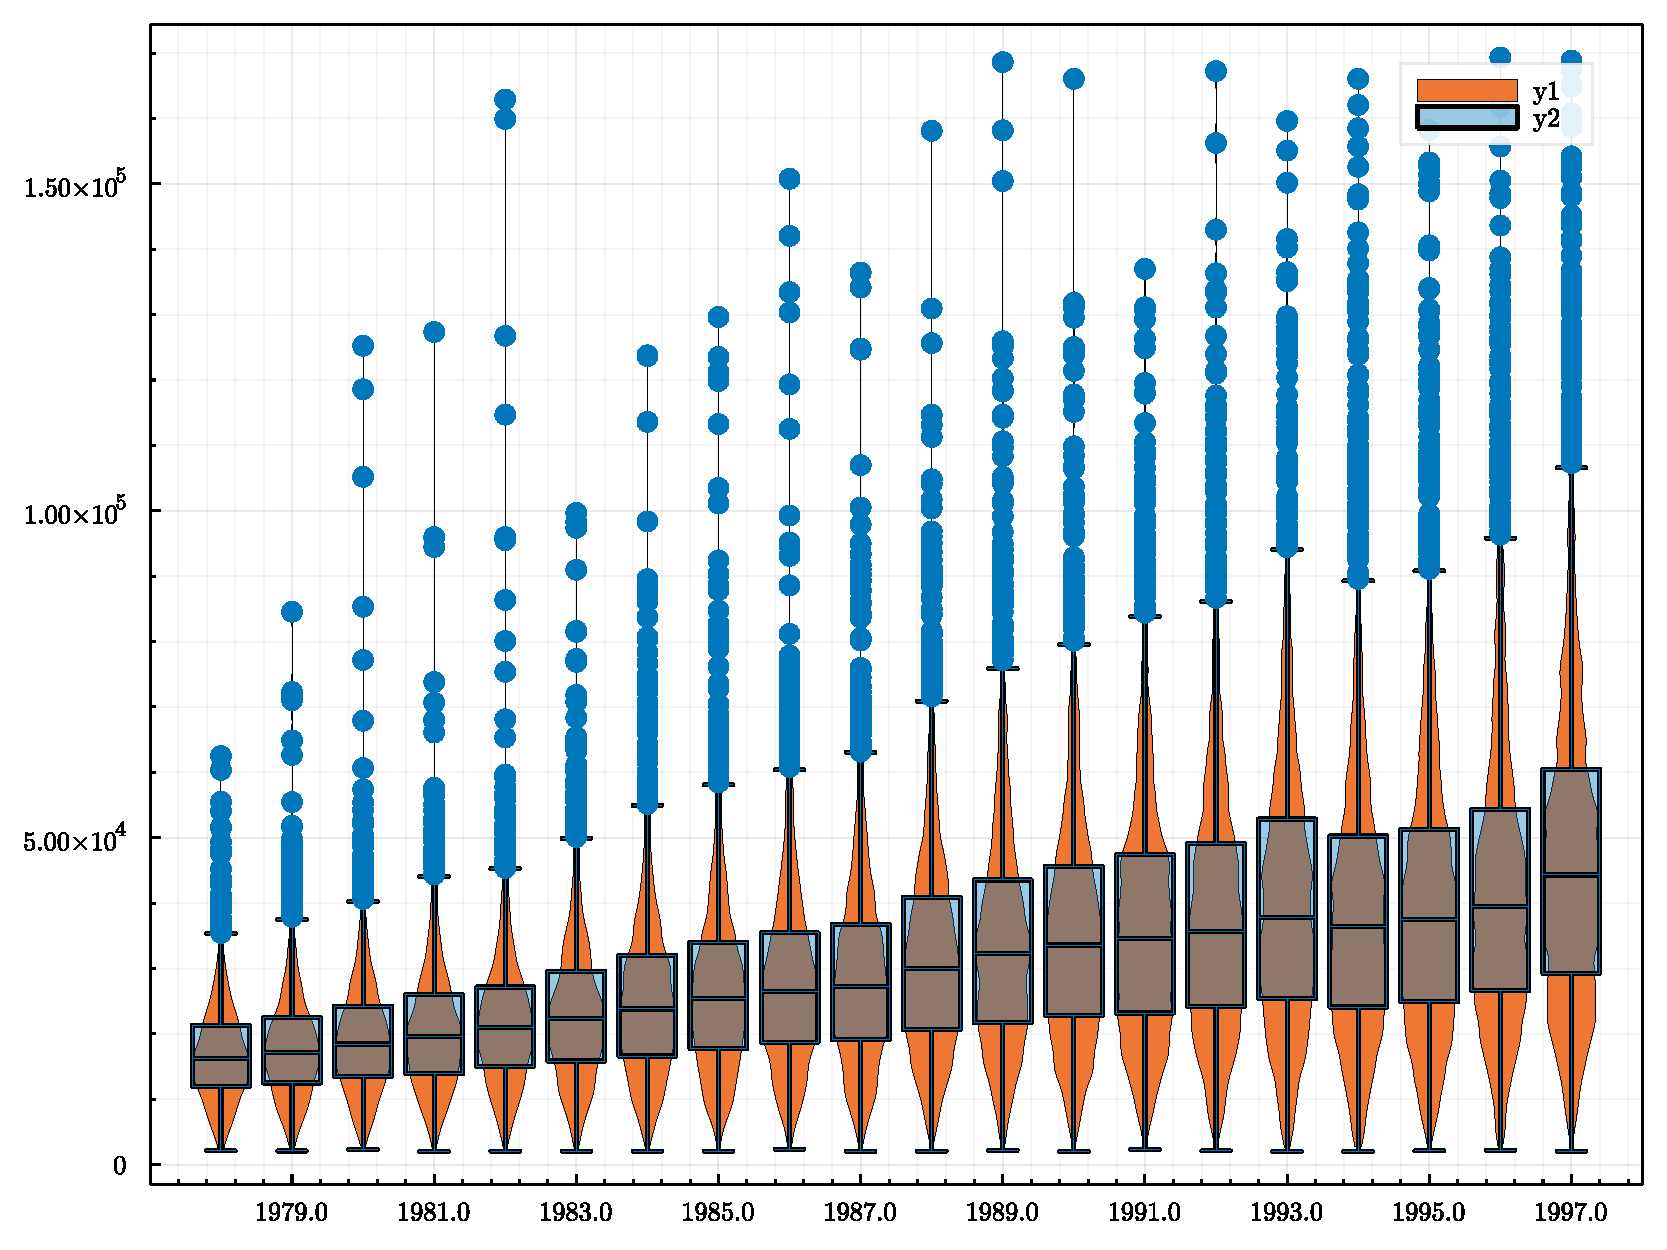
\includegraphics[scale = .5]{04 - 2022 Fall/Econ 810 Advanded Macroeconomic Theory/Part 1/PS 1/document/figures/data_outliers.pdf}
    \caption{Caption}
    \label{fig:my_label}

\end{figure}
After the second transformation the distribution of income looked like 
\begin{figure}[h*]
    \centering
    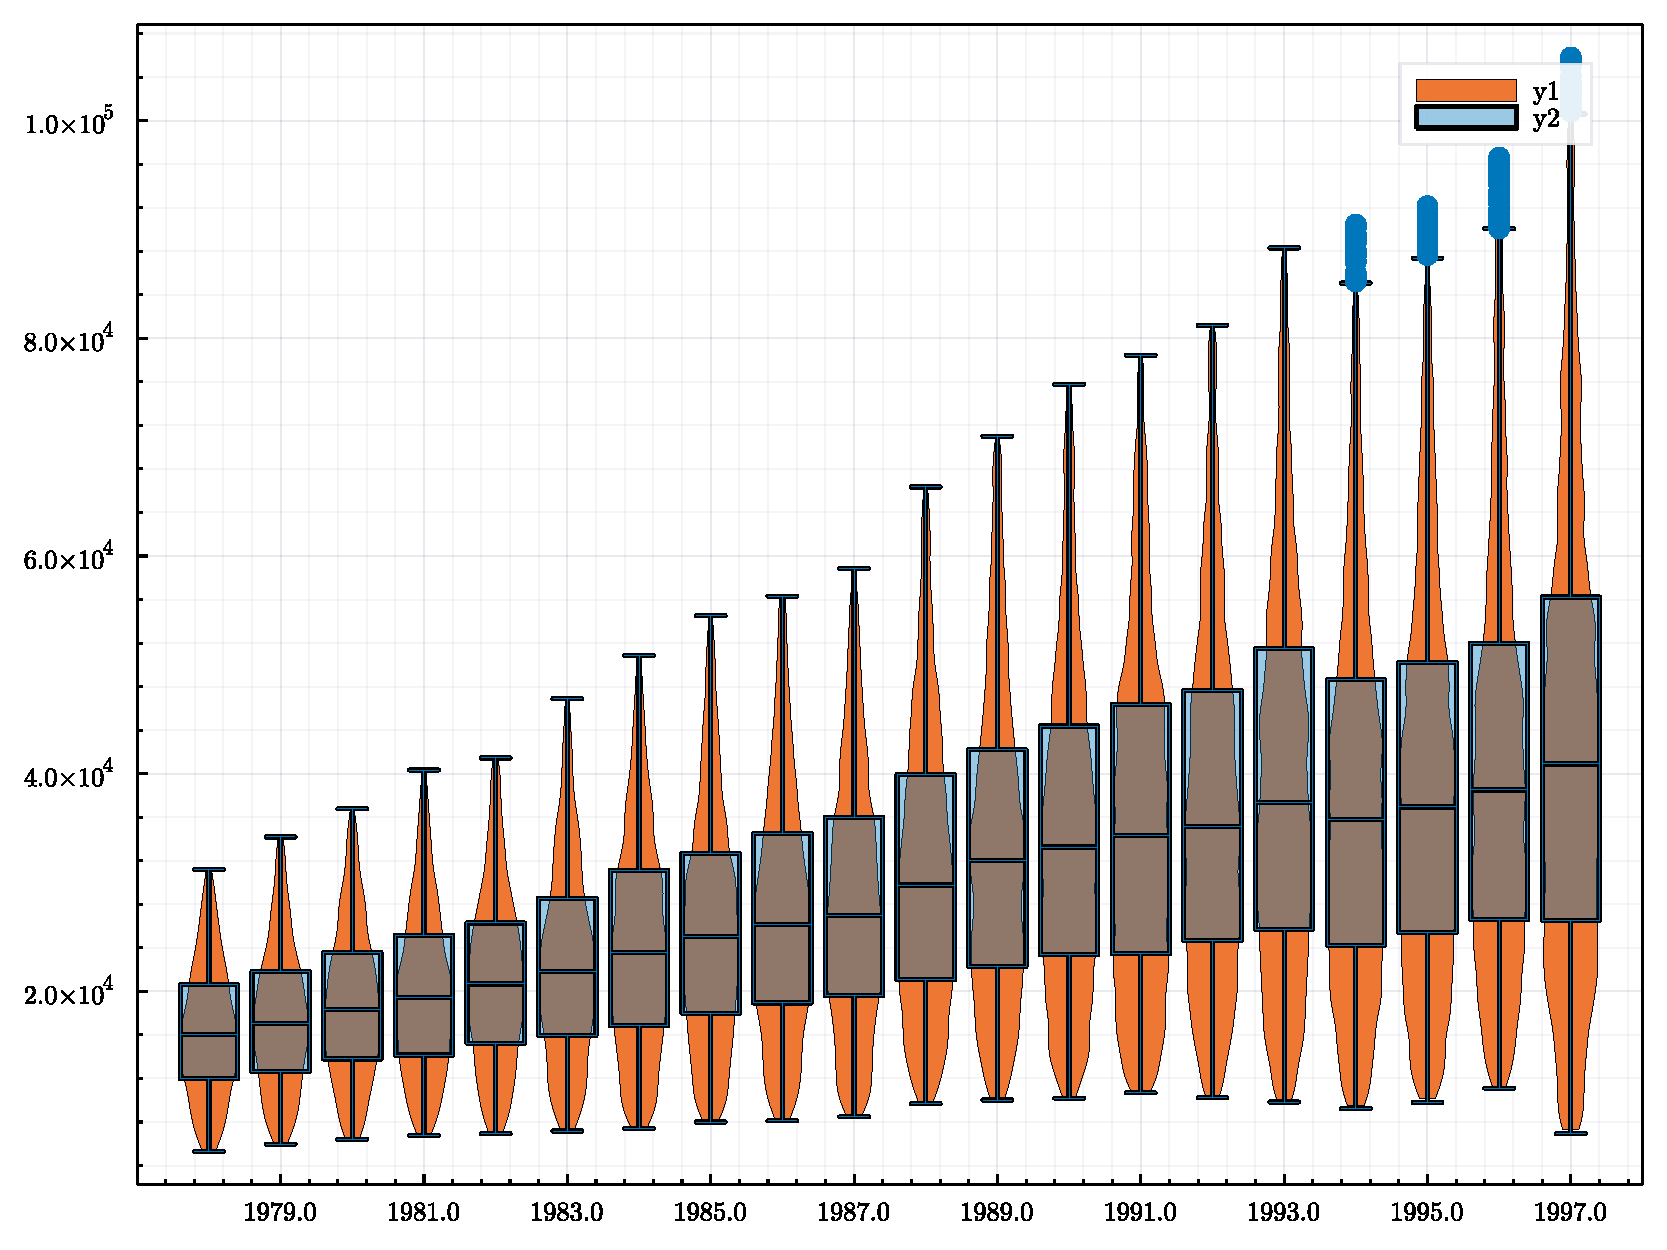
\includegraphics[scale = .5]{04 - 2022 Fall/Econ 810 Advanded Macroeconomic Theory/Part 1/PS 1/document/figures/data_less_outliers.pdf}
    \caption{Caption}
    \label{fig:my_label}
\end{figure}



Assuming that households $i$ receive after-tax income $Y_{i t}$, which takes the form:
\begin{align*}
    \log \left(Y_{i t}\right) &=\kappa_{t}+y_{i t} \\
    y_{i t} &=P_{i t}+\epsilon_{i t}
\end{align*}
where:
\begin{itemize}
    \item $P_{i t}=\rho P_{i, t-1}+\zeta_{i, t}$ , with $\rho<1$ governing the persistence of earnings. 
    \item Persistent shocks, $\zeta$ are such that $\zeta_{i, t} \sim N\left(0, \sigma_{\zeta}\right)$
    \item Temporary shocks $\epsilon$ are such that  $\epsilon_{i, t} \sim N\left(0, \sigma_{\epsilon}\right)$. 
    \item $\zeta_{i, t}$ and $\epsilon_{i, t}$ are independent over time and across households.
\end{itemize}

We can remove the life-cycle component of the income by doing \textcolor{red}{SOMETHING} and we get an age-income profile that looks like:

\begin{figure}[h*]
    \centering
    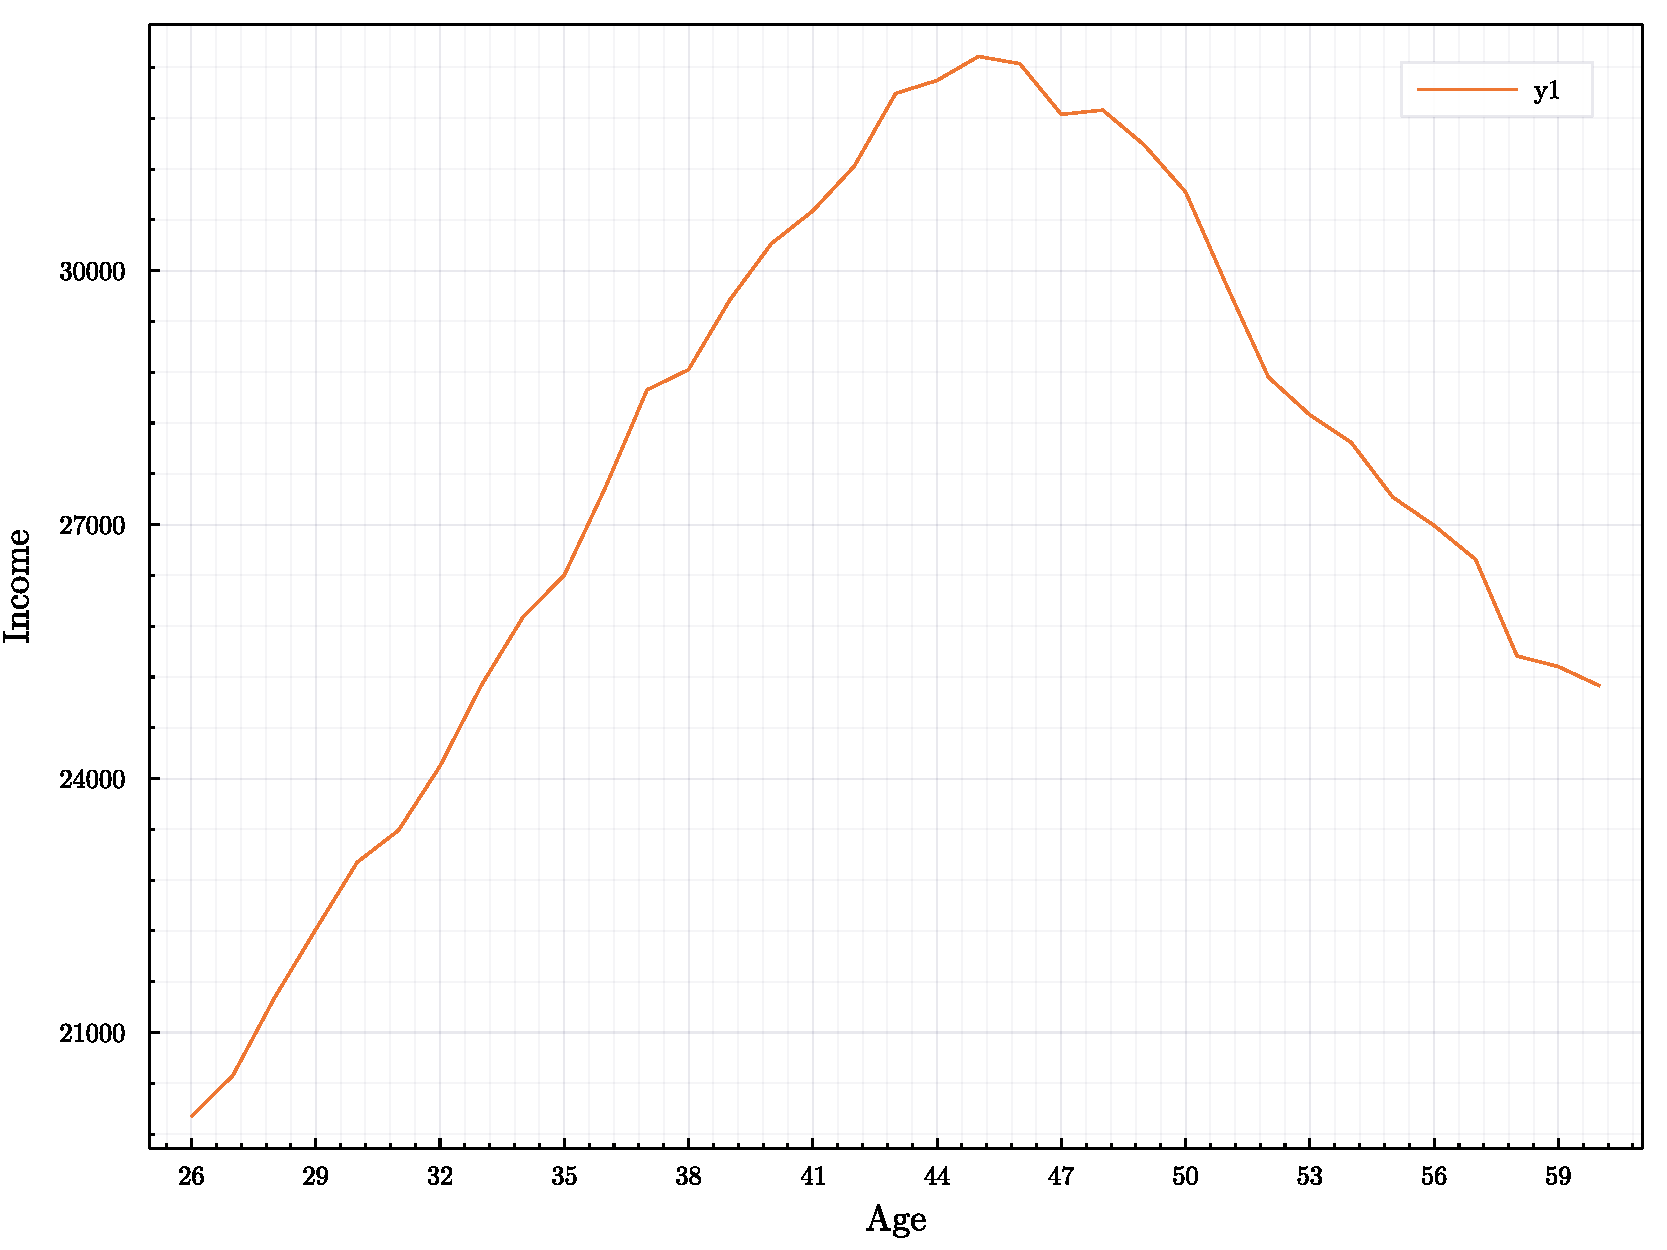
\includegraphics[scale = .5]{04 - 2022 Fall/Econ 810 Advanded Macroeconomic Theory/Part 1/PS 1/document/figures/age_income_profile.pdf}
    \caption{Caption}
    \label{fig:my_label}
\end{figure}

To complete the Data part of this assignment I estimate $\sigma_\varepsilon^2$ and $\sigma_\zeta^2$ using:

$$\textcolor{red}{FORMULAS}$$

\textcolor{red}{table} contains my estimates for different values of $\rho$.

\begin{table}[h*]
    \centering
    \begin{tabular}{|c|c|c|}
        \hline
        $\rho$ & $\sigma_{\varepsilon}^2$ & $\sigma_{\zeta}^2$\\
        \hline
        $0.9$ & $0.079$ & $0.019$\\
        $0.95$ & $0.08$ & $0.018$\\
        $0.97$ & $0.08$ & $0.017$\\
        $0.99$ & $0.08$ & $0.018$\\
        \hline
    \end{tabular}
    \caption{Caption}
    \label{tab:my_label}
\end{table}


\section{Model}
We want to solve the following model:

\begin{align*}\label{810_ps1:seq_problem}
\max_{C_{i,t}, A_{i,t+1}} \quad &\mathbb{E}_0 \sum_{t = 0}^{T}\beta^{t}u(C_{i,t})\\
\text{s.t:} \quad & C_{i,t} + A_{i,t+1} = (1+r)A_{i,t}+Y_{i,t} \qquad \forall t=1,\ldots,T
\end{align*}

we can use the constraint to remove consumption and obtain the following recursive formulation:

\begin{equation}\label{810_ps1:req_problem_naive}
    V^t(A, Y) = \max_{A'}\left\{u\left( (1+r)A+Y - A'\right) + \beta \mathbb{E}\left[ V^{t+1}(A', Y') \mid Y \right] \right\}
\end{equation}

Since $Y_{it}$ depends on the deterministic age-income profile $\kappa_t$ and two stochastic shocks $P_[it]$, $\varepsilon_{it}$ we can write $$Y_{it} = Y(P_{it}, \varepsilon_{i,t}) = \exp{(\kappa_t + P_{it} + \varepsilon_{it})}$$

The we can re-write \eqref{810_ps1:req_problem_naive} in terms of the three states $(A, P, \varepsilon)$ and the choice variable $A'$.

\begin{equation}\label{810_ps1:req_problem}
     V^t(A, P, \varepsilon) = \max_{A'}\left\{u\left( (1+r)A+ Y(P, \varepsilon) - A'\right) + \beta \mathbb{E}\left[ V^{t+1}(A', Y(P', \varepsilon')) \mid P' \right] \right\}
\end{equation}

\subsection{Simulation}

I simulated $5000$ agents over their full life cycle the results of the simulation are summarized in the following two figures:
\begin{enumerate}
    \item \textcolor{red}{figure} represents the average wealth by age,
    \item \textcolor{red}{figure} represents the variance of consumption.
\end{enumerate}

\begin{figure}[h*]
    \centering
    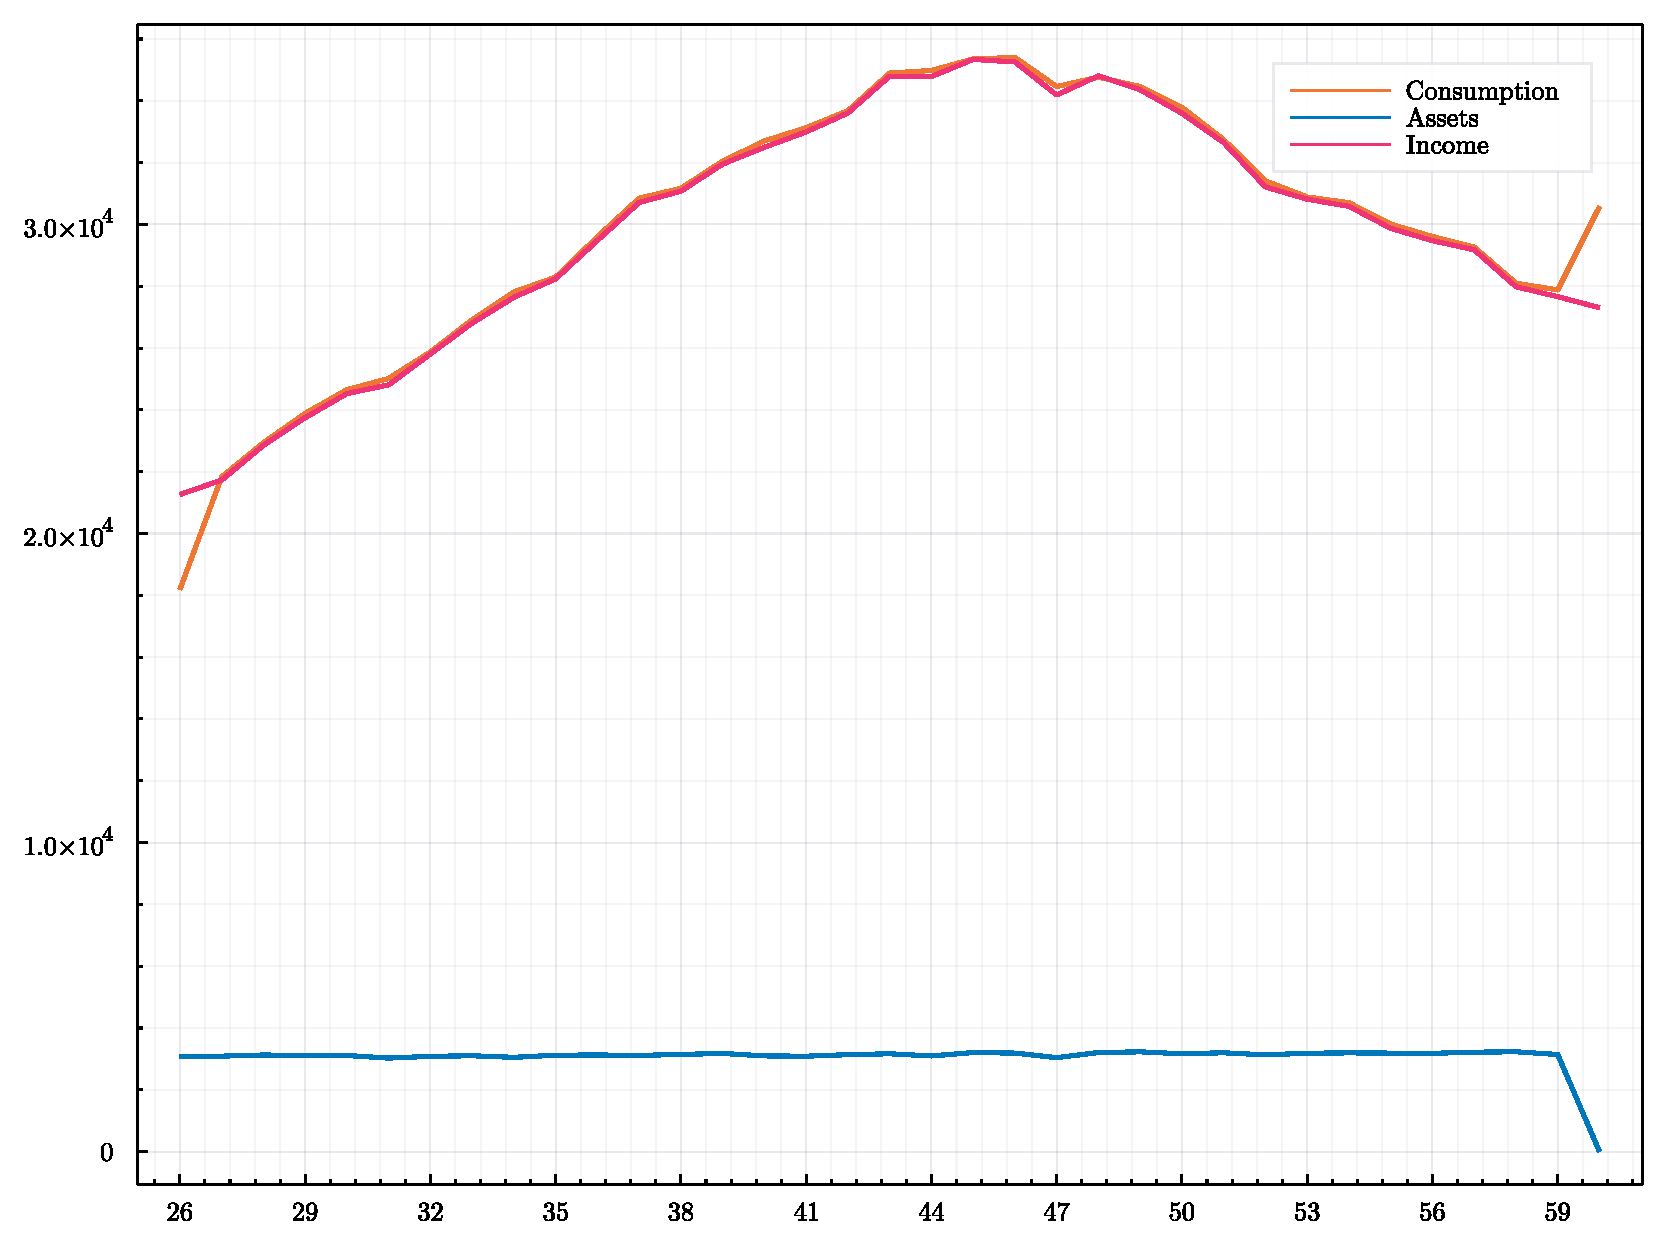
\includegraphics[scale = .5]{04 - 2022 Fall/Econ 810 Advanded Macroeconomic Theory/Part 1/PS 1/document/figures/average_value_of_wealth_by_age.pdf}
    \caption{Caption}
    \label{fig:my_label}
\end{figure}

\begin{figure}[h*]
    \centering
    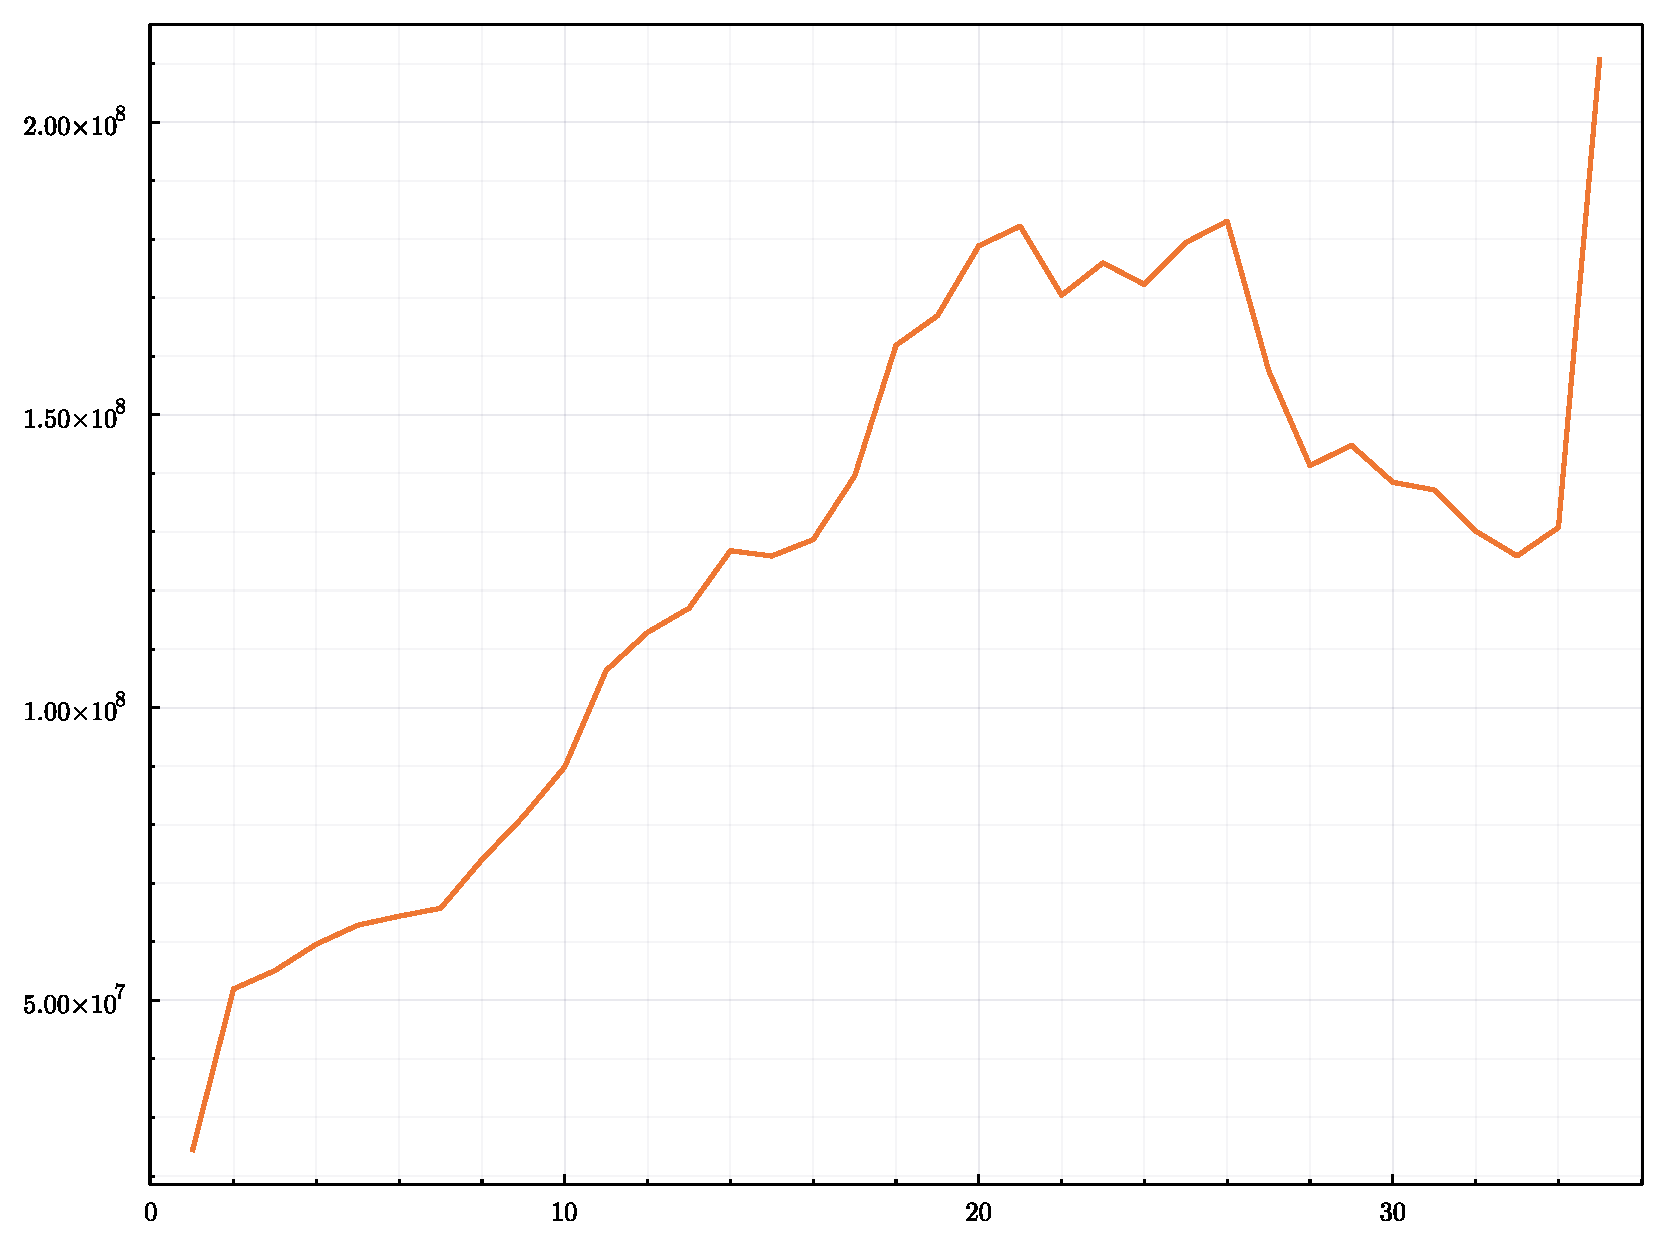
\includegraphics[scale = .5]{04 - 2022 Fall/Econ 810 Advanded Macroeconomic Theory/Part 1/PS 1/document/figures/variance_of_consumption_by_age.pdf}
    \caption{Caption}
    \label{fig:my_label}
\end{figure}



\bibliographystyle{chicago}
\bibliography{references}


\end{document}